\documentclass{standalone}
\usepackage{tikz}
\usepackage{ctex,siunitx}
\usepackage{tkz-euclide}
\usepackage{amsmath}
\usetikzlibrary{patterns, calc}
\usetikzlibrary {decorations.pathmorphing, decorations.pathreplacing, decorations.shapes,}
\begin{document}
\small
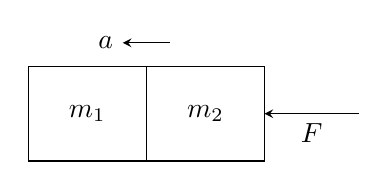
\begin{tikzpicture}[>=stealth,scale=0.6]
  \draw  (0,0) rectangle (5, 2);
  \draw  (0,0) rectangle (2.5, 2);
  \node at (2.5/2,1){$m_1$};
  \node at (2.5+2.5/2,1){$m_2$};
  \draw[<-](5,1)--node [below]{$F$}(7,1);
  \draw[<-](2,2.5)node [left]{$a$}--(3,2.5);
\end{tikzpicture}
\end{document}